% This file was created by matlab2tikz v0.0.7.
% Copyright (c) 2008--2010, Nico Schlömer <nico.schloemer@gmail.com>
% All rights reserved.
% 
% The latest updates can be retrieved from
%   http://www.mathworks.com/matlabcentral/fileexchange/22022-matlab2tikz
% where you can also make suggestions and rate matlab2tikz.
% 
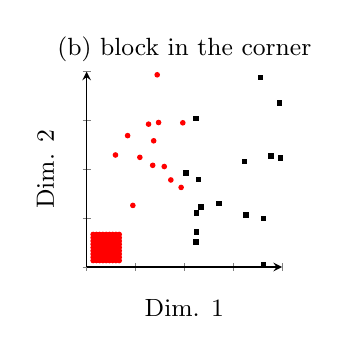
\begin{tikzpicture}

\begin{axis}[
footnotesize,
width= 1.6in,
height= 1.6in,
xmin=0, xmax=30,
ymin=0, ymax=30,
title={(b) block in the corner},
xlabel = {Dim. 1},
ylabel = {Dim. 2},
ytick={0,7.5,15,22.5,30},
xtick = {0,7.5,15,22.5,30},
xticklabels={,,,,},
yticklabels={,,,,},
axis on top,
axis y line = left,
axis x line = bottom
%legend entries={$optimal$,$rand$,$IVM$,$maxent$,$QBC2$,$QBC100$,$SVM$},
 %egend style={nodes=right}
]

\addplot [
color=red,
only marks,
mark=*,
mark options={scale=0.4}
]
coordinates{ (1,1) (1.5,1) (2,1) (2.5,1) (3,1) (3.5,1) (4,1) (4.5,1) (5,1) (1,1.5) (1.5,1.5) (2,1.5) (2.5,1.5) (3,1.5) (3.5,1.5) (4,1.5) (4.5,1.5) (5,1.5) (1,2) (1.5,2) (2,2) (2.5,2) (3,2) (3.5,2) (4,2) (4.5,2) (5,2) (1,2.5) (1.5,2.5) (2,2.5) (2.5,2.5) (3,2.5) (3.5,2.5) (4,2.5) (4.5,2.5) (5,2.5) (1,3) (1.5,3) (2,3) (2.5,3) (3,3) (3.5,3) (4,3) (4.5,3) (5,3) (1,3.5) (1.5,3.5) (2,3.5) (2.5,3.5) (3,3.5) (3.5,3.5) (4,3.5) (4.5,3.5) (5,3.5) (1,4) (1.5,4) (2,4) (2.5,4) (3,4) (3.5,4) (4,4) (4.5,4) (5,4) (1,4.5) (1.5,4.5) (2,4.5) (2.5,4.5) (3,4.5) (3.5,4.5) (4,4.5) (4.5,4.5) (5,4.5) (1,5) (1.5,5) (2,5) (2.5,5) (3,5) (3.5,5) (4,5) (4.5,5) (5,5) (14.7594,22.137) (9.50211,21.9321) (11.9146,15.4247) (4.42475,17.1991) (7.09258,9.45929) (11.0419,22.1845) (14.5021,12.2209) (12.9235,13.3655) (10.8308,29.5065) (10.2906,19.3776) (4.33421,3.57372) (10.1417,15.6132) (6.28981,20.1691) (8.16591,16.8388)
};

\addplot [
color=black,
only marks,
mark=square*,
mark options={scale=0.4}
]
coordinates{ (17.1549,13.4394) (29.7725,16.7571) (16.7772,22.7654) (28.2901,17.0776) (16.8774,8.28907) (17.5203,9.19147) (27.1422,7.43214) (16.8312,5.41786) (20.3286,9.78169) (24.4829,8.00663) (27.1345,0.366002) (29.6109,25.1893) (24.263,16.1932) (15.2474,14.4045) (26.6495,29.111) (16.7822,3.87225)
};

\end{axis}
\end{tikzpicture}
